\documentclass[letterpaper,12pt,twoside=false,DIV=11]{scrbook}

%----------------------CONFIG---------------------------
%math packages
\usepackage{amsmath,amssymb,amsthm,units,unitsdef}
\usepackage{wasysym}  % astro symbols

%bibliography style and citation style, bibstyles to use: plainnat, abbrvnat, unsrtnat, named, chicago
%otherwise numerical citationstyle will be used
\usepackage[authoryear,round]{natbib}
\usepackage{longtable,tabularx,tabulary,multirow,lscape}
\usepackage[font={sl},format=plain,labelfont=bf]{caption}

% appendix
\usepackage{appendix}
\usepackage{xpatch}
\xpretocmd{\appendixpagename}{\sffamily}{}{}

% colors
\usepackage{color,colortbl}
\usepackage[dvipsnames,x11names,svgnames]{xcolor}
\definecolor{darkblue}{HTML}{00354C}

\usepackage{booktabs}
% \usepackage{showkeys} % shows the labels above the references for

%easier development
\usepackage{ifpdf}

\ifpdf
	\usepackage[pdftex]{graphicx}
	\usepackage[]{pdfpages} %for including full pdf pages
	\usepackage[pdftex,
		bookmarks,
		bookmarksopen=true,
		bookmarksnumbered=true,
		pdfauthor={Reto Trappitsch},
		pdftitle={Introduction Arduino},
		colorlinks,
		linkcolor=darkblue,
		citecolor=darkblue,
		filecolor=black,
		urlcolor=darkblue,
		anchorcolor=black,
		menucolor=black,
		breaklinks=true,
		pageanchor=true, %for jumping to a page
		plainpages=false,
		pdfpagelabels=true,
		breaklinks=true]{hyperref}
	\pdfcompresslevel=9
	\pdfoutput=1
	\DeclareGraphicsExtensions{.pdf,.png,.jpg,.jpeg}
\else
	\usepackage{graphicx}
\fi
\usepackage{rotating} % rotate figures
\usepackage{subcaption}
\usepackage{wrapfig}

% break URLs at -
\def\UrlBreaks{\do\/\do-}

%page style
%==========
%\usepackage{geometry}
%\geometry{top=1.0in, bottom=1.0in, left=1.0in, right=1.0in,footskip = 0.5in} 

% Alert boxes
\usepackage{awesomebox}

% Acronyms
\usepackage{acro}
\acsetup{
	make-links = true
}
% THIS FILE CANNOT BE COMPILED ALONE.

% Declare acronyms below in alphabetical order to use with \usepackage{acro}. 

% DECLARE ACRONYMS %

% NUMBERS
\DeclareAcronym{1d}{short = 2D, long = 1 dimensional}
\DeclareAcronym{2d}{short = 2D, long = 2 dimensional}
\DeclareAcronym{3d}{short = 3D, long = 3 dimensional}

% A
\DeclareAcronym{ac}{short = AC, long = alternating current}
\DeclareAcronym{adc}{short = ADC, long = analog-to-digital converter}
\DeclareAcronym{agb}{short = AGB, long = asymptotic giant branch}
\DeclareAcronym{au}{short = AU, long = astronomical unit, short-plural-form=AU}

% B
\DeclareAcronym{bbn}{short = BBN, long = Big Bang nucleosynthesis}
\DeclareAcronym{bh}{short = BH, long = black hole}
\DeclareAcronym{bom}{short = BOM, long = bill of materials}

% C
\DeclareAcronym{cai}{short = CAI, long = calcium-aluminum-rich inclusion}
\DeclareAcronym{ccsn}{short = CCSN, long = core-collapse supernova, short-plural = e, long-plural = e}
\DeclareAcronym{chili}{short = CHILI, long = Chicago instrument for laser ionization}
\DeclareAcronym{cgro}{short = CGRO, long = compton gamma-ray observatory}
\DeclareAcronym{cmb}{short = CMB, long = cosmic microwave background}
\DeclareAcronym{comptel}{short = COMTEL, long = imaging compton telescope}
\DeclareAcronym{cre}{short = CRE, long = cosmic ray exposure}
\DeclareAcronym{csv}{short = CSV, long = comma separated values}

% D
\DeclareAcronym{dac}{short = DAC, long = digital-to-analog converter}
\DeclareAcronym{dc}{short = DC, long = direct current}
\DeclareAcronym{dex}{short = dex, long = decimal exponent}
\DeclareAcronym{doi}{short = doi, long = digital object identifier}

% E
\DeclareAcronym{eagb}{short = E-ABG, long = early asymptotic giant branch}
\DeclareAcronym{ecsn}{short = ECSN, long = electron-capture supernova, short-plural = e, long-plural = e}
\DeclareAcronym{edx}{short = EDX, long = energy-dispersive X-ray spectroscopy}
\DeclareAcronym{esa}{short = ESA, long = European Space Agency}
\DeclareAcronym{euv}{short = EUV, long = extreme ultraviolet}

% F
\DeclareAcronym{frib}{short = FRIB, long = facility for rare isotope beams}
\DeclareAcronym{fip}{short = FIP, long = first ionization potential}
\DeclareAcronym{fit}{short = FIT, long = first ionization time}
\DeclareAcronym{fruity}{short = FRUITY, long = full-network repository of updated isotopic tables \& yields}

% G
\DeclareAcronym{gce}{short = GCE, long = galactic chemical evolution}
\DeclareAcronym{gcr}{short = GCR, long = galactic cosmic ray}
\DeclareAcronym{grb}{short = GRB, long = gamma-ray burst}
\DeclareAcronym{gw}{short = GW, long = gravitational wave}

% H
\DeclareAcronym{hrd}{short = HRD, long = Hertzsprung-Russell diagram}
\DeclareAcronym{hst}{short = HST, long = Hubble Space Telescope}

% I
\DeclareAcronym{icpms}{short = ICP-MS, long = inductively coupled plasma mass spectrometry}
\DeclareAcronym{i2c}{short = I$^{2}$C, long = inter-integrated circuits}
\DeclareAcronym{io}{short = I/O, long = input / output}
\DeclareAcronym{imf}{short = IMF, long = initial mass function}
% \DeclareAcronym{imf}{short = IMF, long = instrumental mass fractionation}
\DeclareAcronym{integral}{short = INTEGRAL, long = international gamma-ray astrophysics laboratory}
\DeclareAcronym{ide}{short = IDE, long = integrated development environment}
\DeclareAcronym{ir}{short = IR, long = infrared radiation}
\DeclareAcronym{irena}{short = IReNA, long = international research network for nuclear astrophysics}
\DeclareAcronym{ism}{short = ISM, long = interstellar medium}

% J

% K

% L
\DeclareAcronym{led}{short = LED, long = light-emitting diode}
\DeclareAcronym{ligo}{short = LIGO, long = laser interferometer gravitational-wave observatory}
\DeclareAcronym{lion}{short = LION, long = laser ionization of neutrals}
\DeclareAcronym{lte}{short = LTE, long = local thermodynamic equilibrium}

% M
\DeclareAcronym{macs}{short = MACS, long = Maxwellian-averaged cross section, short-plural-form = MACS}
\DeclareAcronym{mrsec}{short = MRSEC, long = Materials Research Science and Engineering Center}
\DeclareAcronym{mhdjsn}{short = MHDJSN, long = magneto-hydrodynamic jet supernova, short-plural = e, long-plural = e}
\DeclareAcronym{mesa}{short = MESA, long = Modules for Experiments in Stellar Astrophysics}
\DeclareAcronym{mc}{short = MC, long = Monte Carlo}
\DeclareAcronym{mcmc}{short = MCMC, long = Markov chain Monte Carlo}
\DeclareAcronym{mswd}{short = MSWD, long = mean square weighted deviation}

% N
\DeclareAcronym{nanosims}{short = NanoSIMS, long = nanoscale secondary ion mass spectrometry}
\DeclareAcronym{nlte}{short = NLTE, long = nonplocal thermodynamic equilibrium}
\DeclareAcronym{ns}{short = NS, long = neutron star}
\DeclareAcronym{nse}{short = NSE, long = nuclear statistical equilibrium}
\DeclareAcronym{nupycee}{short = NuPyCEE, long = NuGrid python chemical evolution environment}

% O
\DeclareAcronym{odr}{short = ODR, long = orthogonal distance regression}

% P
\DeclareAcronym{pc}{short = pc, long = parsec}
\DeclareAcronym{pcb}{short = PCB, long = printed circuit board}
\DeclareAcronym{pdfdoc}{short = pdf, long = portable document format}
\DeclareAcronym{pdf}{short = PDF, long = probability density function}
\DeclareAcronym{pn}{short = PN, long = planetary nebula, short-plural = e, long-plural = e}
\DeclareAcronym{pp-chain}{short = pp-chain, long = proton-proton-chain}
\DeclareAcronym{pwm}{short = PWM, long = pulse width modulation}

% Q

% R
\DeclareAcronym{rpproc}{short = \textit{rp}-process, long = rapid proton capture process}
\DeclareAcronym{rgb}{short = RGB, long = red giant branch}
\DeclareAcronym{rims}{short = RIMS, long = resonance ionization mass spectrometry}
\DeclareAcronym{rproc}{short = \textit{r}-process, long = rapid neutron capture process, short-plural = es, long-plural = es}
\DeclareAcronym{rsf}{short = RSF, long = relative sensitivity factor}

% S
\DeclareAcronym{scr}{short = SCR, long = solar cosmic ray}
\DeclareAcronym{sem}{short = SEM, long = scanning electron microscopy}
\DeclareAcronym{sep}{short = SEP, long = solar energetic particle}
\DeclareAcronym{slr}{short = SLR, long = short-lived radionuclide}
\DeclareAcronym{sfr}{short = SFR, long = star formation rate}
\DeclareAcronym{sgb}{short = SGB, long = subgiant branch}
\DeclareAcronym{sic}{short = SiC, long = silicon carbide}
\DeclareAcronym{sims}{short = SIMS, long = secondary ion mass spectrometry}
\DeclareAcronym{soho}{short = SOHO, long = solar and heliospheric observatory}
\DeclareAcronym{sn}{short = SN, long = supernova, short-plural = e, long-plural = e}
\DeclareAcronym{snia}{short = SN-Ia, long = type Ia supernova, short-plural-form = SNe-Ia, long-plural = e}
\DeclareAcronym{snib}{short = SN-Ib, long = type Ib supernova, short-plural-form = SNe-Ib, long-plural = e}
\DeclareAcronym{snic}{short = SN-Ic, long = type Ic supernova, short-plural-form = SNe-Ic, long-plural = e}
\DeclareAcronym{snii}{short = SN-II, long = type II supernova, short-plural-form = SNe-II, long-plural = e}
\DeclareAcronym{sniil}{short = SN-II-L, long = type II-L supernova, short-plural-form = SNe-II-L, long-plural = e}
\DeclareAcronym{sniip}{short = SN-II-P, long = type II-P supernova, short-plural-form = SNe-II-P, long-plural = e}
\DeclareAcronym{sproc}{short = \textit{s}-process, long = slow neutron capture process, short-plural = es, long-plural = es}
\DeclareAcronym{squid}{short = SQUID, long = Simplifying Quantitive Imaging Development and Deployment}
\DeclareAcronym{sw}{short = SW, long = solar wind}

% T
\DeclareAcronym{tec}{short = TEC, long = thermoelectric cooler}
\DeclareAcronym{tisa}{short = Ti:Sa, long = titanium sapphire}
\DeclareAcronym{tdu}{short = TDU, long = third dredge up}
\DeclareAcronym{tof}{short = TOF, long = time-of-flight}
\DeclareAcronym{tpagb}{short = TP-AGB, long = thermally pulsing asymptotic giant branch}

% U
\DeclareAcronym{uv}{short = UV, long = ultraviolet}

% V

% W
\DeclareAcronym{wd}{short = WD, long = white dwarf}
\DeclareAcronym{wmap}{short = WMAP, long = Wilkinson microwave anisotropy probe}
\DeclareAcronym{wr}{short = WR, long = Wolf-Rayet}

% X
\DeclareAcronym{xrb}{short = XRB, long = X-ray burst}

% Y

% Z
\DeclareAcronym{zams}{short = ZAMS, long = zero age main sequence}

%======================================================
% my short cuts
\providecommand{\e}[1]{\ensuremath{\times 10^{#1}}}
\providecommand{\ex}[1]{\ensuremath{^{#1}}}
\providecommand{\dex}[1]{\ensuremath{\delta^{#1}}}
\newcommand{\nean}{$^{22}$Ne($\alpha$,n)$^{25}$Mg}

% textnormal
\newcommand{\tn}{\textnormal}
% textregistered
\newcommand{\tr}{$^\tn{\textregistered}$}

% more box stuff
\providecommand{\boxtitle}[1]{\sffamily{\textbf{#1}}\normalfont}
	
\providecommand{\infobox}[2]{\awesomebox[MidnightBlue]{2pt}{\faPaw}{MidnightBlue}{\boxtitle{#1} #2}}
\providecommand{\morebox}[2]{\awesomebox[BrickRed]{2pt}{\faRocket}{BrickRed}{\boxtitle{#1} #2}}


%======================================================
% My exercise and question environment
\newcounter{exercisecounter}
\setcounter{exercisecounter}{0}
\newcommand{\exer}{Exercise~\theexercisecounter\refstepcounter{exercisecounter}}

\providecommand{\exerbox}[1]{\awesomebox[OliveGreen]{2pt}{\faCode}{OliveGreen}{\boxtitle{\exer} #1}}

\newcounter{questioncounter}
\setcounter{questioncounter}{0}
\newcommand{\question}{Question~\thequestioncounter\refstepcounter{questioncounter}}

\providecommand{\qbox}[1]{\awesomebox[RoyalPurple]{2pt}{\faQuestion}{RoyalPurple}{\boxtitle{\question} #1}}

\newcommand{\cpp}{C\nolinebreak\hspace{-.05em}\raisebox{.4ex}{\tiny\textbf +}\nolinebreak\hspace{-.10em}\raisebox{.4ex}{\tiny\textbf +}}

%======================================================
%title specifications

\title{An Introduction to Building Electronics Projects with Arduino}
\author{Reto Trappitsch}
\date{Fall semester 2021}

%======================================================




%-------------------DOCUMENT---------------------------

\usepackage{blindtext}
\usepackage{listings}

\begin{document}

\lstset{
	language=C++,
	basicstyle=\ttfamily,
	stringstyle=\ttfamily,
	commentstyle=\color{ForestGreen}\ttfamily,
	keywordstyle=\color{NavyBlue}\bfseries,
	frameround=tttt,
	backgroundcolor=\color{AliceBlue},
	morekeywords={
		pinMode, 
		digitalWrite, 
		delay,
		analogWrite
	}
}

\maketitle
% TOC
\pagenumbering{roman}
\setcounter{page}{1}
\tableofcontents

\clearpage


% Chapter numbers
\setcounter{chapter}{-1}

% MAIN TEXT
\pagenumbering{arabic}
\setcounter{page}{1}

\chapter*{Preface}\label{sec:preface}
\addcontentsline{toc}{chapter}{Preface}

The notes are structured into 6 chapters. The first chapter mainly describes basics that students should already know from their introduction to Physics classes. It will be briefly reviewed in the first session. Subsequently, we will discuss one chapter per workshop session. The notes are prepared as we go, and you can always find the latest version, but also solutions to the examples in the form of code examples, on \href{https://github.com/galactic-forensics/workshop_arduino_electronics}{GitHub}. If you find typos, errors, or other issues please let me know. The most recent copy of the \LaTeX\ files and figures can also be found on 

The lecture notes contain clickable links in \textcolor{darkblue}{dark blue}.
Furthermore, boxes throughout the text discuss are used for the following contents:

\infobox{Background information}{on topics that do not necessarily fit into the text but are important to keep in mind will be given in a box like this.}

\morebox{Think about it more!}{These boxes will challenge you to think a problem through for yourself and go into more detail.}

\exerbox{Exercises are given in these boxes. Flex your coding muscles and practize what you've learned.}
\setcounter{exercisecounter}{0}

\qbox{Questions will be given in these boxes. They should solidify your background knowledge.}
\setcounter{questioncounter}{0}

This workshop was first designed for interested students at the \href{https://www.brandeis.edu/mrsec/}{\ac{mrsec}} at Brandeis University in fall 2021. Support is provided by the Brandeis NSF MRSEC, DMR-2011486.

\begin{center}
	\vspace{0.5cm} 
	\href{https://www.brandeis.edu/mrsec/}{
\includegraphics[height=2cm]{graphics/nsf_mrsec_logo.png}}
\end{center}


\printacronyms


% Chapters
%!TEX root = main_arduino_intro.tex

\chapter{Introduction}

Scientific research that focuses on experiments and measurements has rapidly grown in the recent past, mainly thanks to significant improvements in engineering, instrument availability, and computing power. While many companies provide state-of-the-art research instrumentation and setups, cutting-edge scientific discovery often still thrives from home-built setups. 

In addition to scientific instrument developement and availability, the consumer / hobby marked has seen a huge increase in home-made electronics.\footnote{For example, have a look at \href{https://www.nytimes.com/2021/10/10/health/coronavirus-ventilation-carbon-dioxide.html}{this} article in the New York Times. Looking at the images clearly shows a 3D printed case as well as a standard Arduino cloud interface.} This development has especially been facilitated by products such as \href{https://www.arduino.cc/}{Arduinos} and \href{https://www.raspberrypi.org/}{Raspberry Pis}, as well as the huge maker community. Automation of research experiments can often benefit from such existing, low-cost products in order to significantly enhance an experiment or measurement. Furthermore, full low-cost instruments enabling frugal research have also been developed based on such platforms, see, e.g., the \href{https://squid-imaging.org/}{\ac{squid} project}.

\section{Basic Physics to Remember}

Building electroncis is not just fun because you can hold your final product in your hand and play with it, but also since it is a direct application of basic physics. Remember your introductory classes in physics! 

\paragraph{\href{https://en.wikipedia.org/wiki/Ohm's_law}{Ohm's law}} Throughout this workshop, you will encounter Ohm's law very frequently. This law states the current $I$ through a conductor with resisitvity $R$ is directly proportional to the voltage $U$ across the conductor. We can write this as:
\begin{align}
    I &= \frac{U}{R}\\
    U &= RI \label{eqn:uri}
\end{align}
This basic relationship will become really important when designing circuits.

\morebox{Maximum current}{Arduino pins, as we will discover later, can supply 5\,V to, e.g., an \ac{led}. Since an \ac{led} is a diode, it's resistance (if connected properly) is close to zero (see also \href{https://en.wikipedia.org/wiki/Light-emitting_diode}{Wikipedia}). Therefore, applying a 5\,V voltage would result in an infinite current across this component. How would you add a resistor to limit the potential current to a maximum of 10\,mA?}

\paragraph{\href{https://en.wikipedia.org/wiki/Electric_power}{Electric power}} If a current flows through a resistor, electrical energy is transfered. The energy per time that is used in this resistor is the electric power $P$, which can be calculated as
\begin{equation}
    P = U I.
\end{equation}
Often, this electrical power is dissipated as heat. For example, an \href{https://en.wikipedia.org/wiki/Incandescent_light_bulb}{incandescent light bulb} creates light (and heat!) by applying a voltage to a filament that is generally made of tungsten. The filament heats up and emits light. Electronic components generally have a maximum power rating, also often expressed as a maximum current rating.
\morebox{Maximum power versus maximum current}{Assume you have a component that shows tells you a power consumption of at most 5\,W at a current of 1\,A. What is the maximum voltage that you can apply? What is the resistance of this element at this voltage?}

\infobox{Electronic components and symbols}{From your introductory physics class you should be familiar with basic electronic components such as resistors, capacitors, etc., and their symbols. We will discuss various components during this workshop. A good overview of components to refresh your memories can be found \href{https://en.wikipedia.org/wiki/Electronic_component}{here on Wikipedia}. Standard electronic symbols, which are really useful for drawing circuit diagrams, can be found \href{https://en.wikipedia.org/wiki/Electronic_symbol}{here}.}

\section{Analog and Digital}

If you turn on a radio and it is too loud, you can use the volume know, which is nothing else than an adjustable potetiometer, in order to regulate the volume of the sound. This volume can be adjusted over a whole range of settings. The potentiometer adopts linearly depending on its position, giving you an analog control over the volume. Mapping the volume from 0 (quiet) to 1 (loud), you can reach any value in between. Digital signals on the other hand are either on or off. Arduinos generally have many digital \ac{io} pins which can be either high (5\,V) or low (grounded). If you connect a 3.3 V battery to an inpu pin, of course via a resistor in order to not exceed the current maximum, the switch would either tell you that it is high or low, depending on the threshold that are actually set in order to determine this. Any kind of microprocessor \textit{only} understands digital signals. 

\subsection{Analog-to-Digital Conversion}
In order to measure as signal from a sensor, e.g., a photo detector or a temperature sensor as we will use later, a device called \ac{adc} can be used. Above we mentioned that any kind of microprocessor only understands digital signals. The same is also true for an \ac{adc}. While a digital \ac{io} pin has two levels (high / on or low / off), an \ac{adc} generally has many more levels in between. The resolution of an \ac{adc} is generally expressed in bits.

\infobox{Bit}{For any microprocessor, the two possible states (high and low) are generally expressed as 1 and 0. Binary numbers (base 2) are therefore the ideal representation to express different states. A digital \ac{io} pin has 1\,bit resolution, which means it can either be 1 or 0. Higher resolution means that more bits are available to set states. For two bits, i.e., a binary number with with two digits, the possible states are 00, 01, 10, 11. This means that 2\,bit resolution has a total of four steps. For $n$\,bits, the number of available steps are $2^n$.}

\begin{figure}[tb]
    \centering
    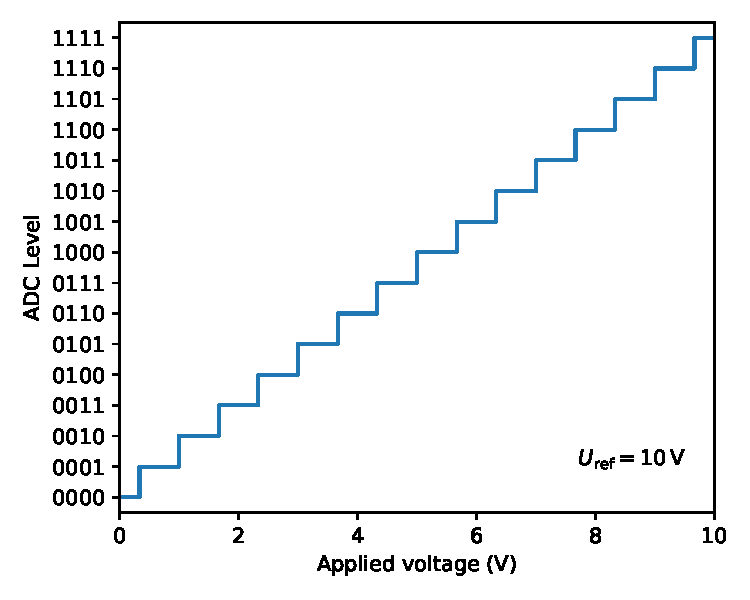
\includegraphics[width=0.625\textwidth]{graphics/00_introduction/adc.pdf}
    \caption{A 4\,bit \ac{adc} with given levels. The reference voltage is 10\,V.}
    \label{fig:intro:adc}
\end{figure}
Figure~\ref{fig:intro:adc} shows the levels of a 4\,bit ADC in binary as a function of the voltage that would be measured. The reference voltage here is $U_\mathrm{ref} = 10\,$V. This reference voltage is the voltage that the \ac{adc} can measure at most, i.e., the voltage that it will return when the \ac{adc} level is $1111$. 

Knowing the resolution $n$ of an \ac{adc}, we can easily calculate the minimum voltage difference that can be determined as 
\begin{equation}
    \Delta U = \frac{U_\mathrm{ref}}{n}.
\end{equation}
For the given example above in Figure~\ref{fig:intro:adc}, the minimum voltage would thus be $\Delta U  = 0.625\,$V. Anything smaller voltage difference requires a higher resolution \ac{adc}.


\subsection{Digital-to-Analog Conversion}\label{sec:intro:dac}

Of course, we sometimes require the opposite of an \ac{adc} and need to convert digital signal into the analog world. The device that allows for this transformation is a \ac{dac}. A true \ac{dac} takes a digital signal and returns an analog voltage by dividing a reference voltage as many times as  necessary. The same resolution limitations as for an \ac{adc} also apply to a \ac{dac}. For example, a 4\,bit \ac{dac} with a reference voltage of $10\,$V can only increase the analog output in steps of 0.625\,V.

\paragraph{\Ac{pwm}} An interesting way to have a pseudo \ac{dac} is to use a process called \acf{pwm}. 
\begin{figure}[tb]
    \centering
    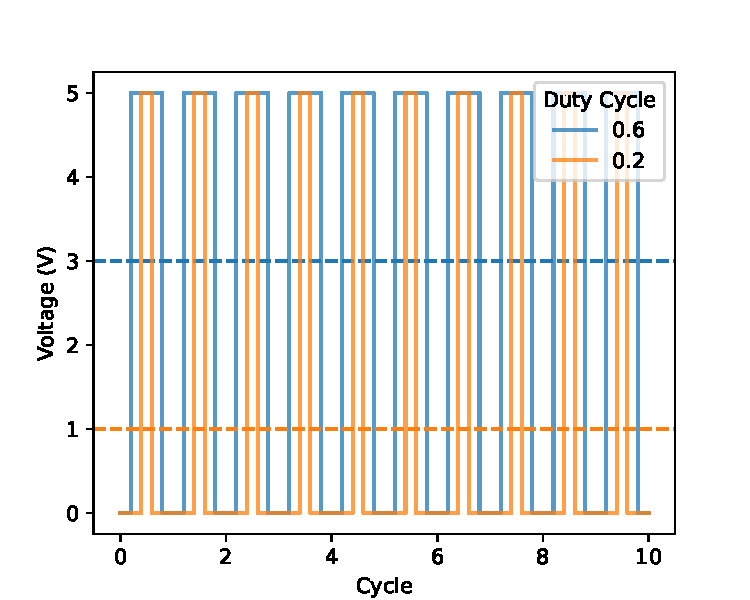
\includegraphics[width=0.625\textwidth]{graphics/00_introduction/pwm.pdf}
    \caption{\Ac{pwm} cycles and average voltage for two different duty cycles.}
    \label{fig:intro:pwm}
\end{figure}
Figure~\ref{fig:intro:pwm} shows a schematic on how this process works with a 5\,V pin. The digital pin is rapidly turned on and off. If it is at 5\,V for 50\% of the time, a 50\% duty cycle, the effective, smoothed-out voltage that can be seen by a ``slow'' component would be 2.5\,V. Depending on the duty cycle, a pseudo-analog output can therefore be created. A great example to use \ac{pwm} is to have a dimmable \ac{led}. \acp{led} generally have only two states, on and off, i.e., is the voltage is high enough to light them, they are bright and otherwise dark. Using \ac{pwm} however, we can turn an \ac{led} on an off in rapid succession such that it looks to the human eye as if the light source itself was dimmed.

\morebox{Analog output with \ac{pwm}}{Can you come up with a way to create a smooth analog output from a \ac{pwm} pin? Think about how your cellphone charger turns \ac{ac} into \ac{dc}.}

\section{Arduino}

For this class, we will be using an Arduino Micro. You can find more information and various alternative arduino boards for all kinds of projects on the \href{https://www.arduino.cc}{Arduino website}.

In Appendix~\ref{app:pinout}, a schematic of the Arduino Micro board is given. This so-called pinout diagram specifies what all the various pins on the board mean and what they are used for. It is a very handy reference for when you develop your project.

\subsection{Programming an Arduino}

The easiest way to program an Arduino is by using the \ac{ide} for Arduino that can be found \href{LINKLINKLINK}{here} \textcolor{red}{LINK}. The website also has installation guides on how to install the IDE and Arduino driver on your computer, depending on your operating system. Please see this documentation or look at it at least briefly, since it will help you with trouble shooting in case your computer does not find the Arduino board.

\paragraph{The Arduino \ac{ide}} is very useful when you are starting to learn how to program your Arduino. Under ``File'', ``Examples'' you can find eleven categories that give you many well-explained example snippets of code for various applications. We will make a lot of use of these examples, especially during the first few chapters of this workshop. The \ac{ide} also allows you to verify your code, i.e., check if it contains any errors (check button in the toolbar) and to upload your code to the Arduino itself (right arrow button in the toolbar). In order to upload your code to the Arduino board, make sure that you have the correct board selected. Go to ``Tools'', ``Board'' to select ``Arduino Micro''. Furthermore, you need to select the port on which your board is connected to the computer. To do so, go to ``Tools'', ``Port'' to select the correct one. Now you are ready to begin uploading example code or your own code.

\paragraph{Programming language overview} To program your Arduino, the code must be written in C++. There are many great introductions online that can help you to get started \textcolor{red}{EXAMPLE LINKS}. Therefore, we will only discuss very briefly the most important basics here. These will help you to avoid the most common mistakes.

\begin{itemize}
    \item Variables must be declared. If you need an integer for example and assign it the value three, you can do this by declaring the variable as \lstinline{int myVar = 3;}
    \item All command lines must be terminated by a semi colon \lstinline{;}
    \item Functions, loops, etc. get surrounded by curly brackets
    \item It is up to the user to make the code look readable. If you want, you can write everything into one line since line endings and function endings are defined by the above stated rules.
    \item Line comments are preceeded with \lstinline{//} while block comments use the following structure:
    \begin{lstlisting}
    /*
        My comments
        in a block...
    */
    \end{lstlisting}
\end{itemize}

In general, the minimum file structure for your Arduino code should look similar to the following.
\begin{lstlisting}[frame=single]
// variable declarations, load libraries

void setup() {
  // setup code

}

void loop() {
  // main code that repeats

}
\end{lstlisting}
On the very top of your code, put variable declarations and initializations if required and load the necessary libraries. The \lstinline{setup} function is the part that runs once when you reset or boot up your Arduino. The \lstinline{loop} function will then run repeatedly and, ideally, until you unplug or reset the Arduino. We will see later how to fill these standard functions. In addition, you can of course write your own functions with any names of your choosing, just make sure they do not collide in naming with these default functions. 

\infobox{Help with programming your Arduino}{To find further information on how to code an Arduino and get yourself started with C++, see the following links \textcolor{red}{ADD LINKS}:
\begin{itemize}
    \item \href{}{Starters guide for programming for Arduino}
    \item \href{}{Reference guide specifically for Arduino}
    \item \href{}{Libraries in Arduino}
    \item \href{}{\dots}
\end{itemize}
Note that many components that we use come with detailed instructions and guides. For example, if you buy components from \href{https://adafru.it}{Adafruit}, these parts generally come with a guide for Arduino, etc.}

\paragraph{More Help}{As with so many things in life these days, more help is generally just one \href{https://www.duckduckgo.com}{search on the internet} away. There are many forums, articles, etc., on the web that discuss building electronics with Arduino. The hope is that this workshop helps you to discover the vast possibilities and gives you the right keywords to search your way through.}

%!TEX root = main_arduino_intro.tex

\chapter{Blink}

Like programming tutorials start with a ``Hello World!'' program, electronics tutorials generally start with a blink example. In this chapter you will learn how to write to and read from digital \ac{io} pins. 

\section{\Acp{led}}

\subsection{Internal \ac{led}}

Arduinos with a built-in \ac{led} allow the user to program and use this \ac{led}. Therefore, all the hardware you need is the Arduino and a USB cable in order to connect it to your computer. Feel free to plug the Arduino into a breadboard as shown in Figure~\ref{fig:blink:arduino_alone}.
\begin{figure}[htb]
    \centering
    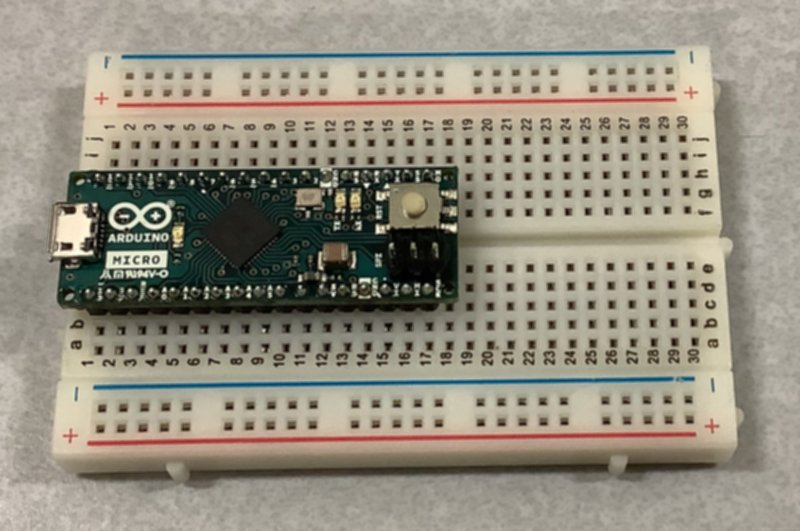
\includegraphics[width=0.6\textwidth]{graphics/01_blink/arduino_alone.jpg}
    \caption{Arduino micro plugged into a breadboard. On the left the USB connection is visible. On the right of the label where it says ``Arduino'', the internal LED can be seen.}
    \label{fig:blink:arduino_alone}
\end{figure}
The internal \ac{led} in Figure~\ref{fig:blink:arduino_alone} can be seen just on the right side of the label that says ``Arduino''. In addition, you can see a button on the right-hand side of the board (the reset button) as well as two more \acp{led} on the left side of this button. These additional \acp{led} cannot be accessed by the user and are reserved for the system.

If you start the \ac{ide} and load the basic example ``Blink'', you will get some code that will control the \ac{led}. The following exercises will use this simple example and slowly extend it.

\exerbox{Open the example blink file and read the comments. What is done in the setup? What does the variable \lstinline{LED_BUILTIN} stand for? Study the loop: What will happen when you upload the code to your Arduino? Do so and see if your assumptions were correct. Modify the timings of the program such that the \ac{led} blinks at a different rate.}

\subsection{External \acs{led}}

We can also connect an external \ac{led} to a digital \ac{io} pin. To use a pin as an output pin, i.e., to set its level by software, we have to define the \lstinline{pinMode} to be in \lstinline{OUTPUT} mode. Furthermore, connecting an \ac{led} to a pin and simply driving it can be bad for the \ac{led}, since it has, by itself, no resistance. Looking at equation~\eqref{eqn:uri} we can see that in such a case the current should become infinity, which might destroy the \ac{io} pin. Fortunately, Arduinos have an internal resistor that prevent this from happening. However, the \ac{led} might still get too much current, which might significantly reduce its lifetime. You can either add a resistor or use an LED with an internal one, as we are doing here (Figure~\ref{fig:blink:arduino_led}).

\begin{figure}[htb]
    \centering
    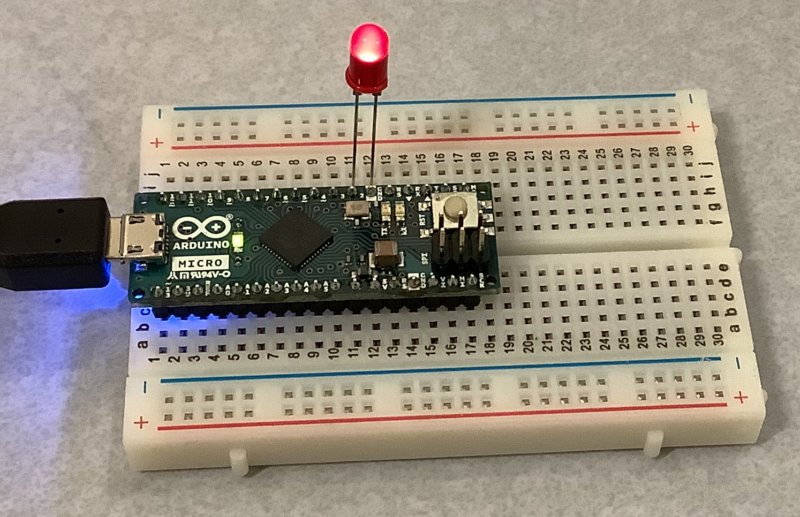
\includegraphics[width=0.6\textwidth]{graphics/01_blink/arduino_led.jpg}
    \caption{Arduino with one \ac{led} connected.}
    \label{fig:blink:arduino_led}
\end{figure}
\exerbox{Draw a wiring diagram to connect your own \ac{led} to a Arduino output pin. Where do the anode and cathode of the \ac{led} connect to? Attach your \ac{led} to the arduino and modify the simple blink experiment to use your \ac{led} instead of the built-in one. If you have trouble figuring out how to connect the \ac{led}, study Figure~\ref{fig:blink:arduino_led} and remember that every electric circiut must be completed.}

\subsection{Dimming an \ac{led}}

As we have discussed above, \acp{led} cannot be dimmed in the traditional way, i.e., by using a potentiometer to lower the voltage. However, we can use a \ac{pwm} output in order to only have the \ac{led} on for a certain amount of time. This will result in our brain perceiving the \ac{led} as dimmed. We have already described the \ac{pwm} outputs above in Section~\ref{sec:intro:dac}, see also Figure~\ref{fig:intro:pwm}. In order to identify a \ac{pwm} output, look at the pinout (Appendix~\ref{app:pinout}). Digital pins indicated with $\sim$ are the ones that can be used in this fashion, e.g., pin 3.

\exerbox{Connect your \ac{led} to a \ac{pwm} output pin. From the Arduino \ac{ide}, load the basic example named ``Fade''.
\begin{enumerate}
    \item Read the setup and loop functions. How is the pin output set and what is different from how the pin was set in the previous exercise?
    \item Modify the fade amount to 7 and run it again. At the brigthest point, the \ac{led} briefly blinks. Why?
    \item Can you rewrite the routine in order to prevent it from blinking at the highest point? An \href{https://www.arduino.cc/reference/en/language/structure/control-structure/if/}{\lstinline{if} statement} might be useful.
\end{enumerate}}

The \lstinline{void loop()} function acts as an endless loop. The most commonly used looping structures are \href{https://www.arduino.cc/reference/en/language/structure/control-structure/while/}{\lstinline{while}} and \href{https://www.arduino.cc/reference/en/language/structure/control-structure/for/}{\lstinline{for}} loops. In fact, the loop function iself underneath is a \lstinline{while(true)} loop.

\exerbox{Inside the \lstinline{void loop()} function, write a \lstinline{for} loop to replace the ramp. Ensure that your loop does not blink, even if you select various fade amounts.}

\qbox{
    \begin{itemize}
        \item How does integer division in \cpp\ work?
        \item How can you do a division in \cpp\ and round the result to the nearest integer?
        \item What is a boolean variable and how do you compare two booleans, e.g., in an \lstinline{if} statement?
        \item How would you flip the state of a boolean variable?
    \end{itemize}
}

\subsection{Multiple \acp{led}}

\begin{figure}[tb]
    \centering
    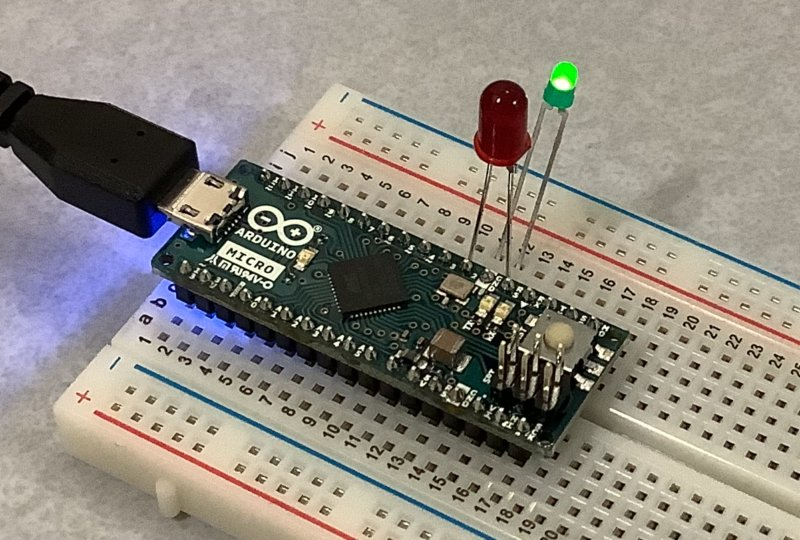
\includegraphics[width=0.5\textwidth]{graphics/01_blink/arduino_two_leds.jpg}
    \caption{An Arduino with two \acp{led} connected.}
    \label{fig:blink:arduino_two_leds}
\end{figure}
Since you have more than one pin available, multiple \acp{led} can be set up. An example of a test setup is shown in Figure~\ref{fig:blink:arduino_two_leds} This can be especially useful if you want to display the status of your setup using different colored \acp{led}.

\paragraph{Subfunctions in \cpp} Sometimes it is useful to put some of your code into external functions, i.e., not to write them into the main loop. For example, you can write a function as following:

\begin{lstlisting}
void myFunction(bool toggle) {
    // your code here...
}
\end{lstlisting}
You can then call this function from the main loop by calling \lstinline{myFunction(true);} if you want to assign the value \lstinline{true} to the variable \lstinline{toggle}.

\exerbox{Setup two \acp{led}, a red and a green one. Write a program that switches between blinking the red and green \acp{led}. Write a subroutine that takes a boolean variable as an input and, depending on the value of this input variable, turns either the red or the green \ac{led} on (and the other one off).}

\section{Buttons}

\begin{figure}[tb]
    \centering
    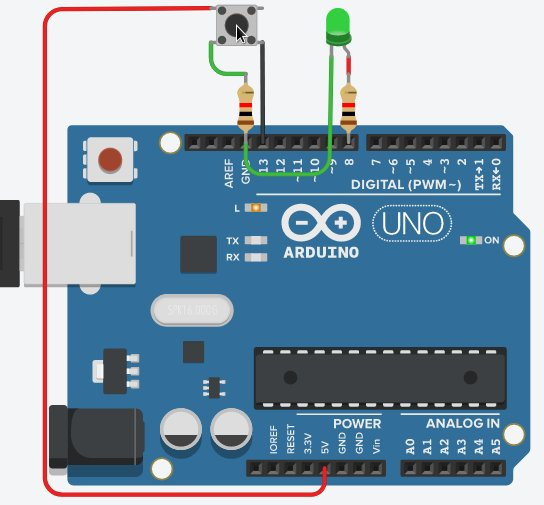
\includegraphics[width=0.45\textwidth]{graphics/01_blink/arduino_button_led_tinkercad.jpg}
    \caption{\href{https://www.tinkercad.com/things/5VP2mIHUOxB}{TinkerCAD simulation} of Arduino with a button and \ac{led} connected.}
    \label{fig:intro:button_led}
\end{figure}
Most devices that allow for user interactions contain some buttons. We can use the digital \ac{io} pins in order to connect a button. Figure~\ref{fig:intro:button_led} shows a \href{https://www.tinkercad.com}{TinkerCAD} simulation of an Arduino with a button and an \ac{led} connected. Here, we connect the button on one side to the 5\,V output of the Arduino and the other side via a 1\,k$\Omega$ resistor to ground and simultaneously to a digital \ac{io} pin. The resistor limits the current to 5\,mA, see equation~\eqref{eqn:uri}. In the setup routine, we need to set the \lstinline{pinMode} to \lstinline{INPUT}, since we want to read the value that is connected to the pin. If the button is unpressed, the pin is on the same electrical potential as ground and therefore in a low state. If the button is pressed however, the pin is at 5\,V and thus in a high state. In the loop you can, e.g., read the state of the button connected to \lstinline{buttonPin} as:
\begin{lstlisting}
int buttonState = digitalRead(buttonPin);
if (buttonState == HIGH) {
    // the button is pressed
} else {
    // the button is not pressed
}
\end{lstlisting}

\exerbox{Connect a button and an \ac{led} to your Arduino and write a program that turns the \ac{led} on while the button is pressed. Then adjust your routine such that, whenever you press the button, the \ac{led} is turned on for 3\,s and then turns off after the time has elapsed.}

\morebox{Adding time}{In the second part of the above exercise, you have (most likely) written your program such that if the button is pressed while the \ac{led} is on, nothing happens. The light will still turn off once the set time elapses after the initial button press. Can you come up with code that would allow you to reset the countdown when pressing the button again, i.e., add time to the timer?}


% Bibliography

% TODO: Clean the bilbliography up

% \phantomsection
% \addcontentsline{toc}{chapter}{Bibliography} \label{sec:bibliography}
% \bibliographystyle{aasjournal}
% \bibliography{origin_elements}

% Appendix
\clearpage
\appendix
\addappheadtotoc
\appendixpage
\clearpage

%!TEX root = main_arduino_intro.tex

\chapter{Arduino Micro Pinout}\label{app:pinout}

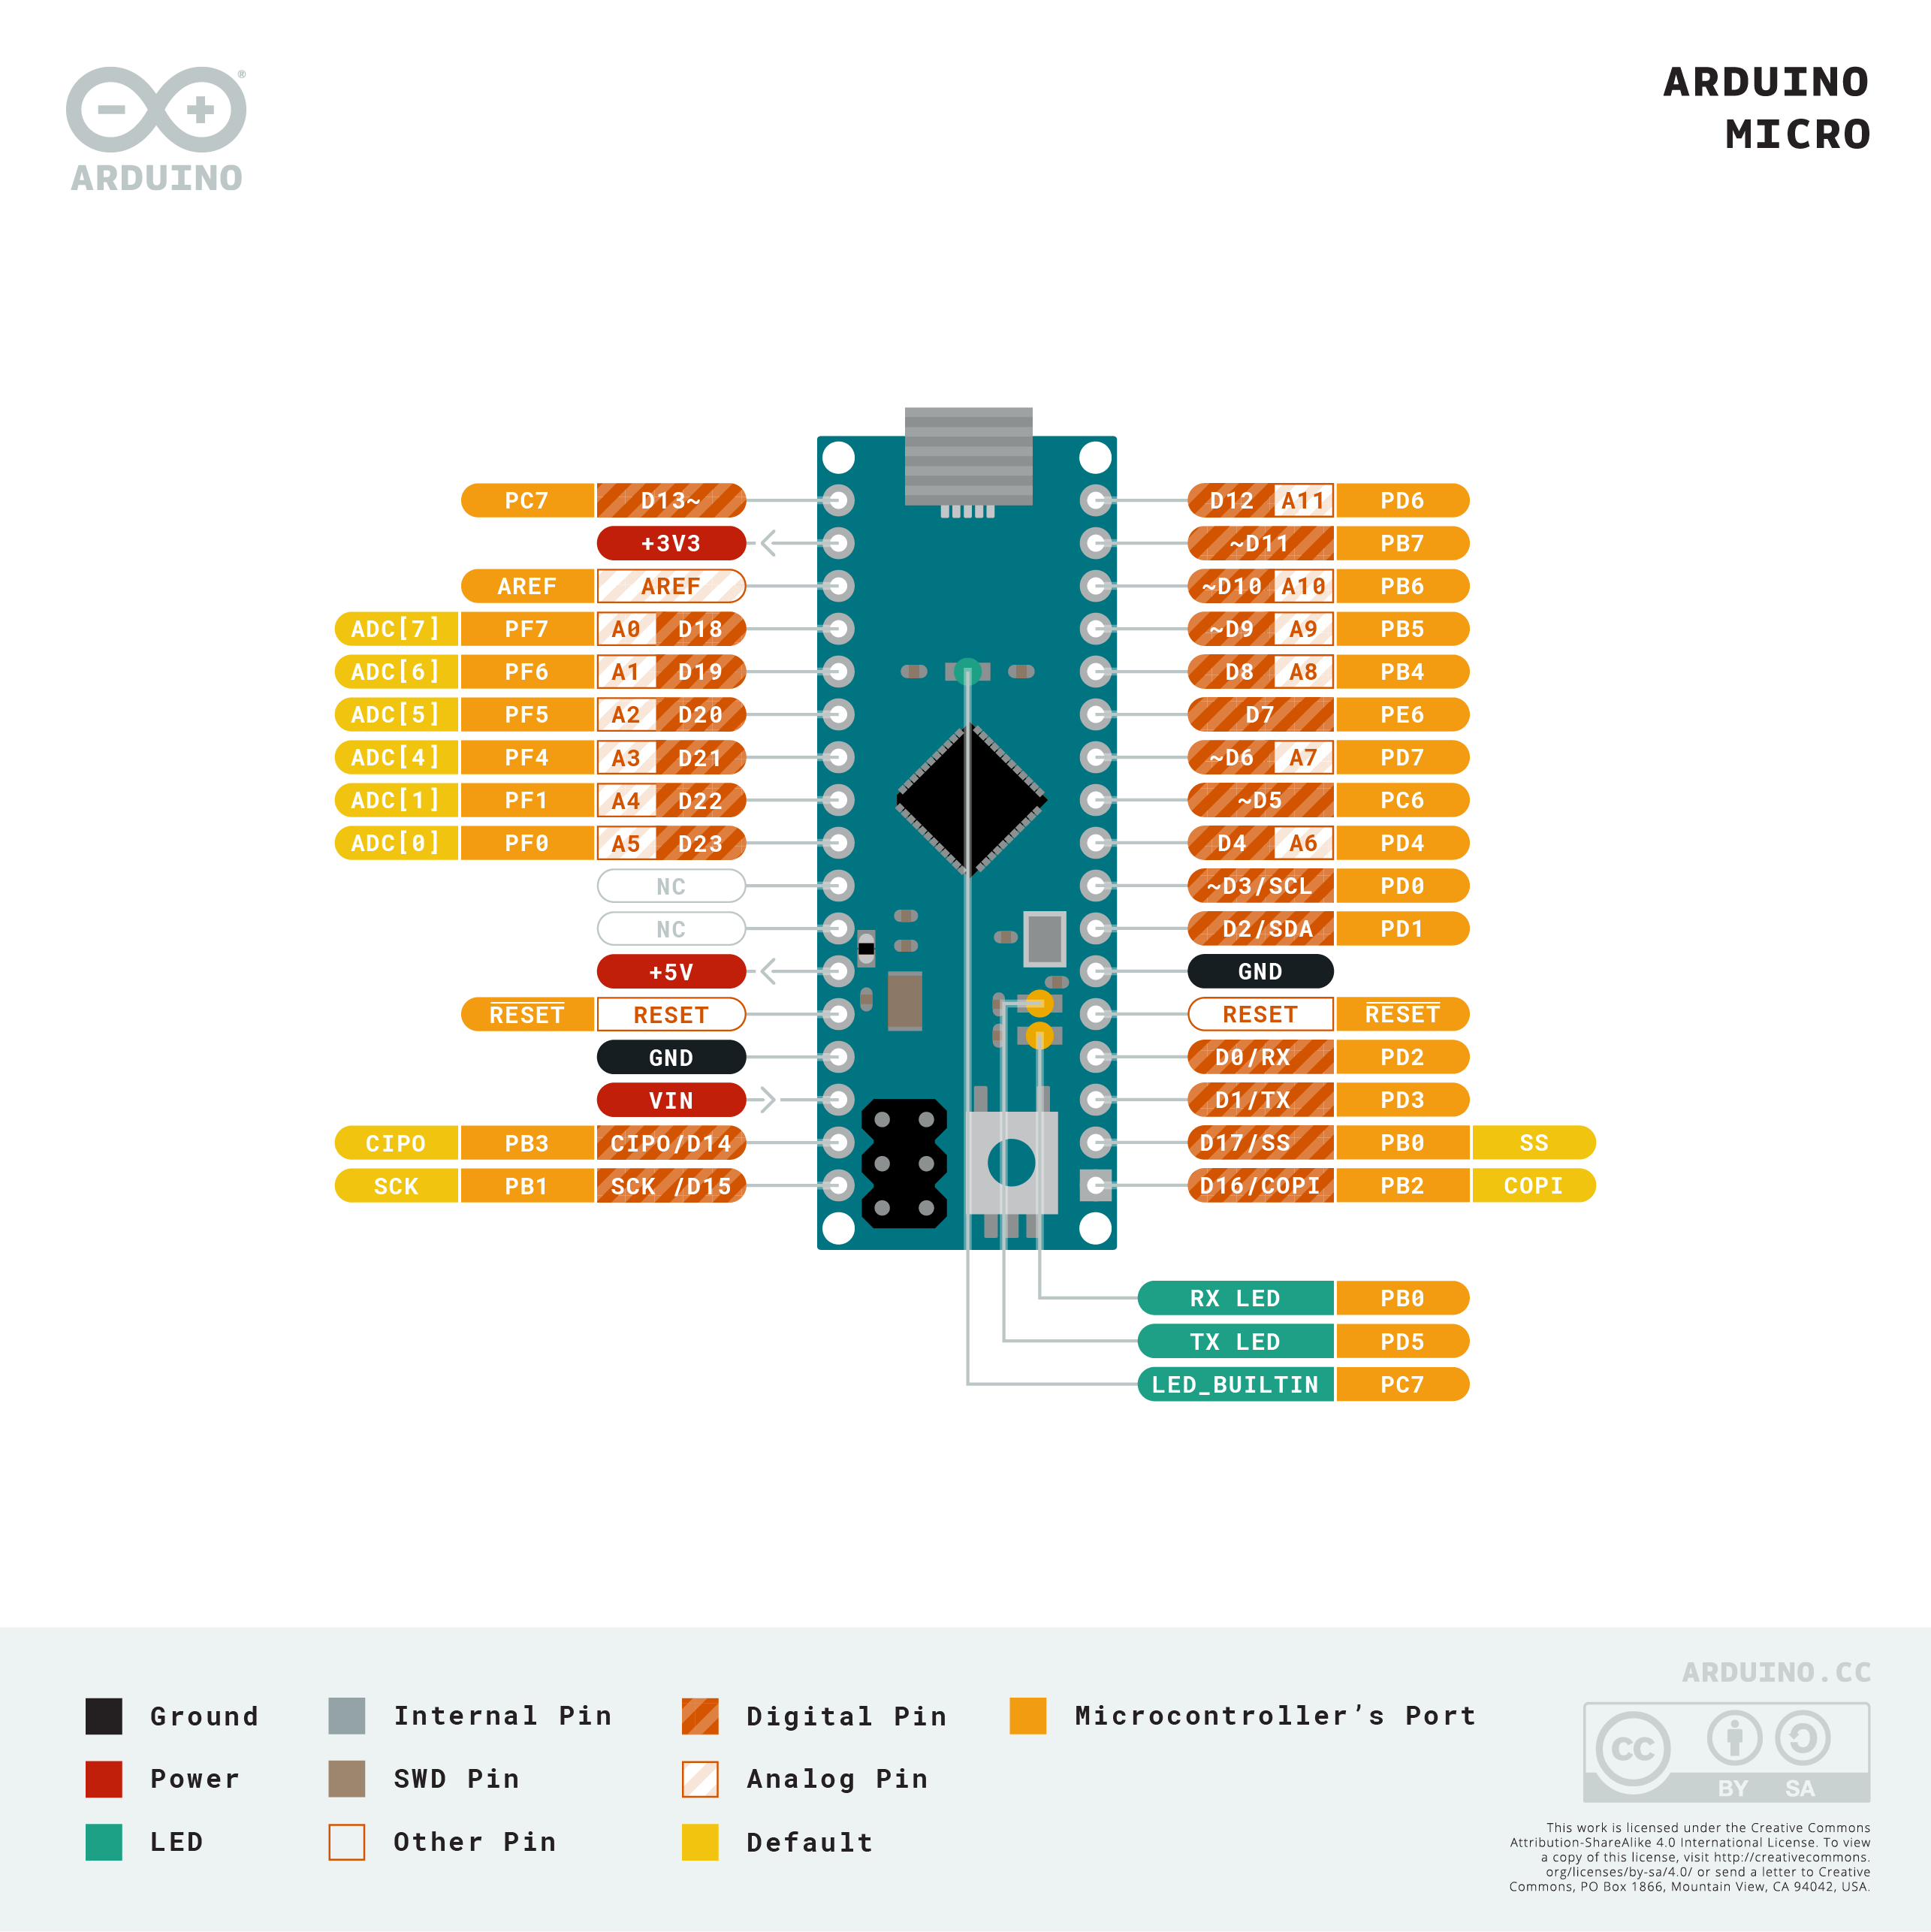
\includegraphics[width=\textwidth]{graphics/appendix/arduino_pinout.png}

%%%%%%%%%%%%%%%%%%%%%%%

\chapter{\Acf{bom}}

The following table states all components used in this workshop. It assumed that soldering stations and supplies are provided.

\begin{center}
\begin{tabular}{lllcr}
\hline
\textbf{Component}  &   \textbf{Supplier}   &   \textbf{Article \#} &   \textbf{Amount} &   \textbf{Cost total} \\
\hline\hline
Arduino Micro       &   \href{https://www.digikey.com/en/products/detail/arduino/A000053/4486332}{Digikey}             &   A000053             &   1   &   \$20.70 \\
USB Cable           &   \href{https://www.digikey.com/en/products/detail/cui-devices/CBL-UA-MUB-1/9838595?s=N4IgTCBcDaIIwAYwFoCsBOALAZmQOQBEQBdAXyA}{Digikey}             &   102-5943-ND         &   1   &   \$2.55 \\
Breadboard          &   \href{https://www.adafruit.com/product/239}{Adafruit}   &   239     &   1   &   \$5.95  \\
Breadboard wires    &   \href{https://www.adafruit.com/product/153}{Adafruit}   &   153     &   1   &   \$4.95  \\
\ac{led} red        &   \href{https://www.digikey.com/en/products/detail/broadcom-limited/HLMP-3600/637603?s=N4IgTCBcDaIKwEYBsBaBBmdBOFA5AIiALoC%2BQA}{Digikey}    &   516-1339-ND         &   1   &   \$0.81  \\
\ac{led} green      &   \href{https://www.digikey.com/en/products/detail/broadcom-limited/HLMP-3962/637598?s=N4IgTCBcDaIKwEYBsBaBBmdAWFA5AIiALoC%2BQA}{Digikey}     &   516-1334-ND &   1   &   \$0.78 \\
Buttons             &   \href{https://www.adafruit.com/product/367}{Adafruit}   &   367     &   1   &   \$2.50  \\
Resistors 1\,k$\Omega$ & \href{https://www.adafruit.com/product/4294}{Adafruit}  &   4294    &   1   &   \$0.75  \\
Resistors 10\,k$\Omega$ & \href{https://www.adafruit.com/product/2784}{Adafruit}  &   2784    &   1   &   \$0.75  \\
Display             &   \href{https://www.adafruit.com/product/1002}{Adafruit}   &   1002    &   1   &   \$10.95    \\
Thermistor          &   \href{https://www.adafruit.com/product/372}{Adafruit}   &   372     &   1   &   \$4.00  \\
\Ac{tec}            &   \href{https://www.adafruit.com/product/1335}{Adafruit}   &   1335    &   1   &   \$34.95     \\
MOSFET              &   \href{https://www.adafruit.com/product/355}{Adafruit}   &   355     &   1   &   \$1.75  \\
12\,V power supply  &   \href{https://www.adafruit.com/product/352}{Adafruit}   &   352     &   1   &   \$24.95     \\
Power jack adapter  &   \href{https://www.adafruit.com/product/368}{Adafruit}   &   368     &   1   &   \$2.00  \\
\hline
\textbf{Total cost:}    &   &   &   &   \textbf{\$118.34}   \\
\hline
\end{tabular}
\end{center}

%%%%%%%%%%%%%%%%%%%%%%%

\chapter{Open source design tools}

\section{Calculators}
\begin{itemize}
    \item \textbf{Heat sink calculator} to determine if you need a heat sink or not. \url{https://daycounter.com/Calculators/Heat-Sink-Temperature-Calculator.phtml} 
\end{itemize}

\section{Designing}
\begin{itemize}
    \item \textbf{EasyEDA}{Online designer for \acp{pcb} with large library of components and direct ordering possibilities. \url{https://easyeda.com/}}
    \item \textbf{Fritzing} Makes electronics design accessible. Easy and simple interface to draw some of your own setups, quick to get started with. Suppliers such as Adafruit have Fritzing libraries with components that you can import. \url{https://fritzing.org/}
    \item \textbf{KiCad} Cross-platform electronics design suite. \url{https://www.kicad.org/}
\end{itemize}

\section{Virtual Hardware}
\begin{itemize}
    \item \textbf{TinkerCAD} Electronic playground from Autodesk. Allows you to virtually set up electronic components and write / test code for them. \url{https://www.tinkercad.com/}
\end{itemize}

%%%%%%%%%%%%%%%%%%%%%%%

\chapter{Full wiring diagram}

\begin{figure}[h!]
    \centering
    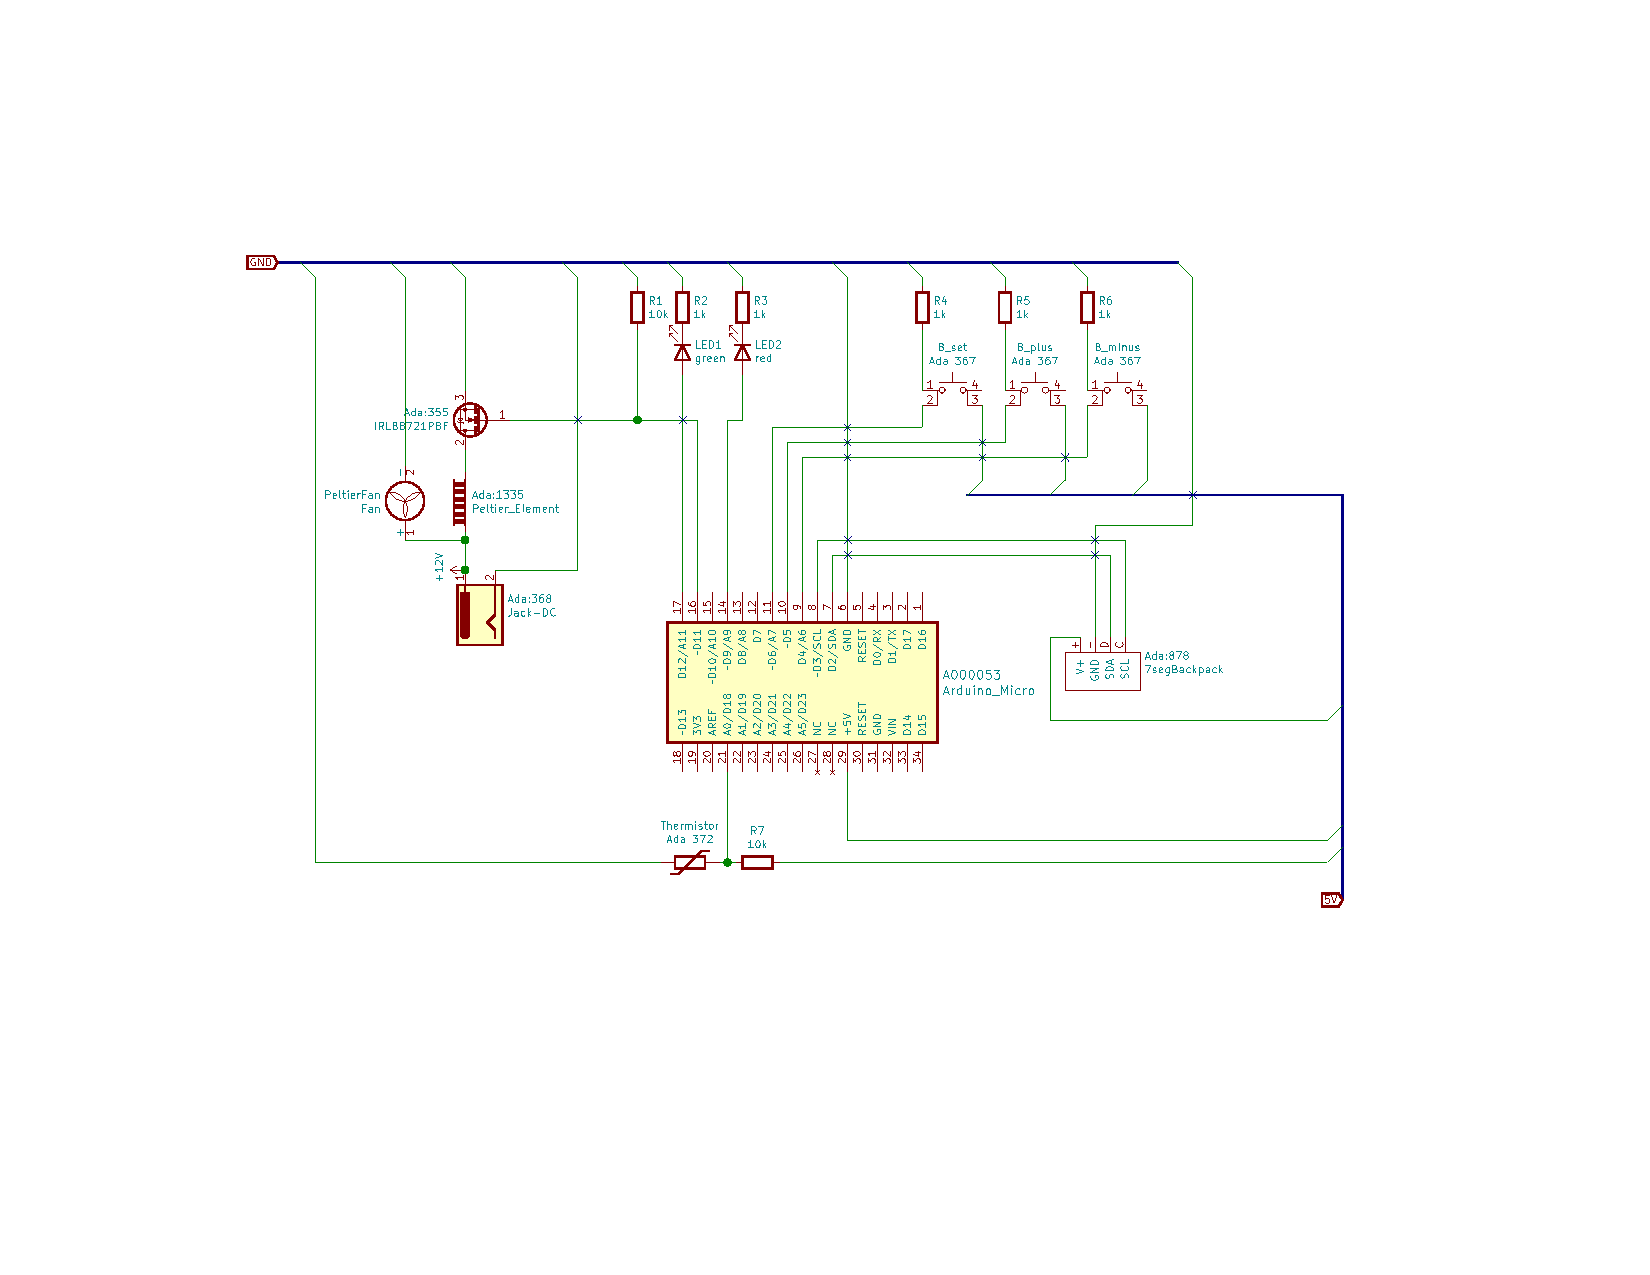
\includegraphics[width=\textwidth]{graphics/appendix/diagram_full_assembly.pdf}
    \caption{Full wiring diagram of the final project. All \href{https://www.kicad.org/}{KiCAD} files can be found on \href{https://github.com/galactic-forensics/workshop_arduino_electronics/tree/main/kicad}{GitHub}.}
    \label{fig:appendix:full_wiring_diagram}
\end{figure}


\end{document}